\documentclass[12pt]{article}
\usepackage{graphicx}
\usepackage{xcolor}
\usepackage{subfigure}
\usepackage[margin=1.0in]{geometry}
\usepackage{float}
\usepackage{ulem}
\usepackage{amsmath}
\usepackage{mathtools}
\usepackage{wrapfig}
\renewcommand{\baselinestretch}{1.5}
\usepackage[utf8]{inputenc}
\author{Shivesh Pathak}
\title{Developing effective theories for the square lattice Hubbard model using density matrix downfolding}

\begin{document}
\maketitle
\begin{abstract}
A core problem of condensed matter physics is understanding how to systematically develop low-energy effective models for strongly correlated electron systems. 
We believe that a density matrix downfolding (DMD) method can be used to systematically build effective theories for such systems beginning with a high energy theory like the \textit{ab-initio} Hamiltonian H$_\text{ab}$.
We present as a preliminary result an effective theory developed using DMD which can accurately reproduce the spectra and properties of the lowest lying excitations of the CuO molecule.
As a step towards bulk strongly correlated materials, we propose developing effective theories using DMD for the simplest toy system which exhibits strongly correlated behavior: the 1-band square lattice Hubbard model at half-filling for various couplings U and temperatures T.
\end{abstract}
Committee: Lucas Wagner, ...
\pagebreak

\section{Introduction}
Systematically developing model Hamiltonians which can accurately describe the energies and properties of the lowest lying eigenstates for strongly correlated electron systems is a pressing problem in modern condensed matter physics. 
At the forefront of modern research are materials such as the cuprate supercondutors, heavy fermion systems, and most recently, twisted bilayer graphene (TBLG).
These materials exhibit various phases of matter which are far from understood, like unconventional superconductivity, psuedogap and bad metal phases, quantum critical points, and stripe ordering.
While no definitive models for these phases have been introduced, it is expected that strong correlations between electronic degrees of freedom lead to these phases.

The necessity for non-perturbative, many-body models in describing the low-lying excited states of strongly correlated electron systems poses a difficult challenge when developing effective theories for real world systems.
Consider for now just the case of TBLG, where for certain magic twist angles, bands near the Fermi surface flatten out to a bandwidth of O(10) meV.
At these magic angles, a small doping can lead to superconductivity and many-body insulating phases in the material, indicative of electronic interaction effects which cannot be explained by a simple band theory.
The effects of the interaction are also beyond just simple renormalization of the non-interacting parameters in a band theory.
A non-perturbative, many-body effective theory is therefore necessary to describe these interesting phases in TBLG.

Common approaches to building suitable model Hamiltonians for strongly correlated materials involve using single particle theories like density functional theory (DFT).
One-body terms are typically obtained by projecting the solutions from the DFT band structure onto a localized single-particle basis, giving an estimate of hoppings and occupations on a lattice model.
Two-body terms in the model are developed by assuming a screened Coulomb interaction based on constrained DFT or RPA.
Aside from this method, L\''{o}wdin methods coupled to a stochastic method and canonical transformations have also been used to develop effective theories.
These methods have the drawback that the constructed effective theory typically does not come with any estimate of the quality of the model, therefore making model validation a phenomenological task which can lead to unclear biases in the model construction.

I propose using a quantum Monte Carlo (QMC) density matrix downfolding (DMD) procedure to develop accurate many-body effective theories for single (SLG) and bi-layer graphene (BLG) systems as a step towards building a many-body model for the strongly correlated TBLG system.
DMD is a relatively new method which allows one to systematically downfold the \textit{ab-initio} Hamiltonian for a system to a many-body lattice model.
While it can be applied to any system, the methods necessary to carry out the downfolding accurately and efficiently have not yet been developed and tested for strong correlated materials.
Both BLG and SLG provide useful playgrounds for developing methods for DMD since they have moderate interaction effects, with non-interacting theories describing the lowest lying excitations relatively accurately.
Fitting models for SLG and BLG from DMD will not only provide a useful stepping stone towards understanding TBLG, but will also help mature the DMD method for its application to other strongly correlated systems.

\section{Methods}
\subsection{Density Matrix Downfolding (DMD)}
We begin by defining what we mean by a low-energy effective Hamiltonian and downfolding.
Consider a Hamiltonian $\hat{H}$ defined on a Hilbert space $\mathcal{H}$.
A low-energy effective Hamiltonian is an operator $\hat{H}_\text{eff}$ which can accurately reproduce the spectra, up to a constant, and eigenstates of $\hat{H}$ on a subpsace $\mathcal{LE}$ of the Hilbert space $\mathcal{H}$.
Here $\mathcal{LE}$ is taken to be the span of the N lowest energy eigenstates of $\hat{H}$, and $\hat{H}_\text{eff}$ is a linear combination of Hermitian operators $\hat{d}_k$ with a constant energy shift $E_0$
\begin{equation}
\hat{H}_\text{eff} = \sum_{k} g_k \hat{d}_k  + E_0.
\label{eq:Heff}
\end{equation}
The objective of Hamiltonian downfolding is to construct such an $\hat{H}_\text{eff}$ given $\hat{H}, \mathcal{H}$.

The key insight of DMD is that the Hamiltonian downfolding problem can be mapped onto a linear regression problem.
It has been shown that the above definition of $\hat{H}_\text{eff}$ is equivalent to the following: a low-energy effective Hamiltonian is an operator on a subspace $\mathcal{LE}$ of $\mathcal{H}$ such that 
\begin{equation}
\begin{split}
\forall |\Psi\rangle \in \mathcal{LE},\ (E[\Psi] \equiv \langle \Psi|\hat{H} | \Psi \rangle)  = \\ (E_\text{eff}[\Psi] \equiv \langle \Psi | \hat{H}_\text{eff} | \Psi \rangle) + \epsilon[\Psi]
\end{split}
\label{eq:DMD}
\end{equation}
where $\epsilon[\Psi]$ is the error in the effective theory.
Given the general linear form of $\hat{H}_\text{eff}$ seen in \eqref{eq:Heff}, 
the task of building an effective Hamiltonian then reduces to fitting a linear model that minimizes the error $\epsilon[\Psi]$ over $\mathcal{LE}$.
The independent variables (descriptors) in the fitting are expectation values of the operators $d_k[\Psi] \equiv \langle \Psi |\hat{d}_k|\Psi \rangle$ and the target variable is $E[\Psi]$.

This linear regression problem can be tackled in three steps, beginning with sampling states from $\mathcal{LE}$.
Ideally the linear regression would be conducted over the entire space $\mathcal{LE}$. 
In practice, the space is too large, and instead a representative sample set is drawn and used for fitting.
For each sampled state $|\Psi_s\rangle$, the quantities $E[\Psi_s], \{d_k[\Psi_s]\}$ are calculated to be used in the linear regression.
Optimal sampling schemes vary between systems and can significantly reduce the number of samples required to achieve robust statistics.

Generally, however, one cannot sample the true low-energy subspace and low-energy wave functions are sampled from an approximate subspace $\mathcal{LE}^\prime$.
A model fit to an arbitrary subspace of $\mathcal{H}$ will generally fail in describing the low-energy excitations of $\hat{H}$.
Rather, the choice of approximate subspace must be made carefully to ensure the fit model is transferable to the true low-energy space.
We describe in detail later how we selected $\mathcal{LE}^\prime$ for the CuO molecule and the scheme used to draw samples from it.

Next, a set of candidate descriptors which form the effective Hamiltonian are selected.
Descriptors will typically be selected if their values co-vary with the energy over the set of sampled states. 
Knowledge of the low-energy degrees of the freedom from experiment and physical intuition can help restrict the set of candidate descriptors further.
In principle there is no restriction on the form of the candidate operators other than Hermiticity, but second quantized operators are commonly used.

Typically, candidate operators are written in second quantized form, and an appropriate single particle basis to express these operators must be constructed.
An appropriate choice of single particle basis can simplify the representation of the effective theory and typically depends on the system of interest.
Common choices include Bloch waves and molecular orbitals for delocalized basis elements or Wannier and intrinsic atomic orbitals for localized ones.
The selected single particle basis can be validated by ensuring it accurately describes single particle properties among the sampled states like the total number of electrons in the system.

Finally, the sampled data are used to fit the coefficients $\{g_k\}$ by linear regression.
A typical fitting workflow involves feature selection, model regression and model validation.
Feature selection methods for choosing appropriate descriptors can range from wrapper methods like orthogonal matching pursuit and principal component analysis to embedded methods like LASSO, ridge and elastic net regularizations. 
Fitting the effective Hamiltonian usually involves an ordinary least squares linear regression, but the cost function can be altered as in the cases of the embedded methods above or weighted least squares linear regression.
Model validation can be carried out by calculating cross validated single parameter measures like R$^2$ scores which carry information about goodness of fit and overfitting.

Importantly, the fit effective Hamiltonian carries with it a quantitative measure of its validity.
The ability to quantify the accuracy of an effective Hamiltonian sets DMD apart from contemporary downfolding approaches which typically report only a final model.
Given the statistical nature of the fitting procedure, model quality assessment can be carried out and reported in exhaustive detail if one is interested.
Typically, however, simple single parameter measures like cross validated R$^2$ scores and root mean squared errors are used to quantify the accuracy of the effective Hamiltonian.

\subsection{Fixed-node diffusion Monte Carlo (FN-DMC)}
Diffusion Monte Carlo (DMC) is a quantum Monte Carlo method which projects out the ground state of a real-space Hamiltonian given some initial trial wave function.
Consider a trial wave function $|\Psi_T\rangle$ and the Hamiltonian $\hat{H}$ with ground state $|\Phi_0\rangle$. 
Applying the projector $e^{-\tau \hat{H}}$ as $\tau \rightarrow \infty$ to $|\Psi_T \rangle$
\begin{equation}
\lim_{\tau \rightarrow \infty} e^{-\tau \hat{H}} |\Psi_T\rangle 
\equiv \lim_{\tau \rightarrow \infty} |\Psi_\text{DMC}(\tau)\rangle \propto \langle \Phi_0|\Psi_T\rangle |\Phi_0\rangle,
\end{equation}
projects out the ground state as long as the trial wave function is not orthogonal to the ground state. 
DMC provides a stochastic implementation of this projector method and involves moving samples from the trial function $\Psi_T(R)$ using the Green function $G(R, R^\prime, \tau) = \langle R | e^{-\tau(\hat{H} - E_T)} | R^\prime \rangle$. 
Since $\hat{H} = \hat{T} + \hat{V}$, kinetic and potential energy terms, the Green function is approximated by a Trotter expansion $G(R, R^\prime, \tau) = \langle R | e^{-\tau(\hat{H} - E_T)} | R^\prime \rangle \sim \Big[e^{-d\tau(\frac{V(R) + V(R^\prime)}{2} - E_T)} \langle R| e^{-d\tau\hat{T}}|R^\prime \rangle + O(d\tau^2) \Big]^N $ where $d\tau = \tau/N$.
This expansion can be interpreted as an interative procedure where samples are moved N times with a small timestep $d\tau$ until convergence.
The constant $E_T$ is a trial energy used to control the normalization of $\Psi_\text{DMC}(\tau, R)$ and is updated at each move.

DMC, however, suffers from a fermion sign problem which is alleviated via a fixed-node approximation.
Under the fixed-node approximation the nodal surface of $\Psi_\text{DMC}(\tau, R)$ is forced to match that of the initial trial wave function for all $\tau$.
This approximation makes FN-DMC variational, and will only return the exact ground state of $\hat{H}$ if the nodal surfaces of $|\Psi_T\rangle$ and $|\Phi_0\rangle$ are identical.

We take advantage of the variational nature of FN-DMC to sample the low-energy states necessary for DMD.
Consider a set of trial wave functions with varying nodal structures.
The final projected $\Psi_\text{DMC}$ for these different trial functions will be the lowest energy states in $\mathcal{H}$ for the given nodal structures.
If the initial trial wave functions are appropriately chosen, the final projected states will be low-energy states within $\Psi_\text{DMC}$.
We calculate the expectation values $E[\Psi_\text{DMC}], \{d_k[\Psi_\text{DMC}]\}$ necessary for the model regression using a mixed estimator.
Details for calculating reduced density matrix elements in FN-DMC can be found in Wagner.

\section{Preliminary Work}
\subsection{Non-orthogonal determinants in FN-DMC trial wave functions}
In order to become acquainted with our code QWalk \cite{WAGNER20093390} and QMC algorithms in general I worked on implementing and testing multi-Slater-Jastrow trial functions with optimized non-orthogonal determinants (MSJ+NO) in FN-DMC \cite{Pathak2018}.
We assessed the efficiency and compactness of this new trial function by calculating the ground state energy and single particle densities of a C$_2$ molecule using FN-DMC and comparing to the results when using multi-Slater-Jastrow trial functions with optimized orthogonal determinant trial functions (MSJ+O). 
The workflow involved constructing the un-optimized trial wave functions, optimizing the parameters using an energy optimization method \cite{Toulouse2007}, and finally using the optimized trial functions in both variational Monte Carlo (VMC) and FN-DMC calculations. 
We found the average improvement in variational energy when using optimized orthogonal determinants is $\langle E_\text{MSJ} - E_\text{MSJ+O} \rangle = $ 0.32 eV with a standard deviation of 0.08 eV, with an additional improvement from the non-orthogonal determinants of 0.031 eV with a standard deviation of 0.021 eV.
The average improvement in the FN-DMC energy with the MSJ+O trial wave functions was 0.14 eV (standard deviation 0.03 eV) with an additional reduction of 0.032 eV (standard deviation 0.019 eV) when using the MSJ+NO trial wave function.
While the benefit using the MSJ+NO trial wave function seems small, we saw that the FN-DMC energy calculated using an MSJ+NO trial function with only 24 determinants was lower than the FN-DMC energy using an MSJ+O trial function with 55 determinants.
Further, the FN-DMC charge density calculated using MSJ+NO trial functions had stronger bonding character than when using MSJ+O trial functions, a reasonable result as introducing correlations into trial functions allows for electrons to avoid each other while still occupying the same bonding region. 
Our results indicated that using non-orthogonal determinants may lead to more compact multi-Slater-Jastrow trial wave functions for small molecules.

\subsection{Effective theory for CuO molecule using DMD}
As a first step towards developing accurate models for extended systems like solids using DMD, we constructed a many-body effective model for the CuO molecule which accurately describes the eigenstates and spectra seen in experiment up to 2eV above the ground state.
The neutral CuO molecule has been a subject of intense theoretical and experimental study due to the complex structure of its low-energy space.
While the low-energy excitations in the doublet sector of the CuO molecule are well understood, singlet selection rules for spectroscopic measurements and the doublet ground state leave the quartet sector of excitations unexplored.
We construct our $\mathcal{LE}$ based on recent anion photoelectron spectroscopy (APES) measurements of the low-lying excited states of the nuetral CuO molecule. 
The lowest lying excitations involve electrons in the Cu 3d, Cu 4s and O 2p orbitals.
Given that the lowest energy excitations contain a fully-filled Cu 3d shell or a single hole in this shell we define our low-energy space as:
\begin{equation}
\mathcal{LE} = \text{Span(}\{ |\Psi \rangle | \langle \Psi | \hat{n}_{3d} | \Psi \rangle \ge 9,\ \hat{H}_\text{ab}|\Psi\rangle = E |\Psi\rangle \}\text{)}.
\label{eq:LE}
\end{equation}

Our sample space was generated by using multi-Slater-Jastrow trial wavefunctions in FN-DMC.
The parameterization for our low-energy trial wave functions was
\begin{equation}
e^{J}\sum_{i} c_i|\text{D}_i\rangle = \sum_{i} c_i (e^J |\text{D}_i \rangle) \xrightarrow{FN-DMC} \ \sim \sum_i c_i |\Phi_i \rangle \in \mathcal{LE}
\label{eq:sampling}
\end{equation}
where $e^J$ is a three-body Jastrow factor and $|\text{D}_i\rangle$ is a Slater determinant whose nodes accurately approximate those of an eigenstate $|\Phi_i \rangle \in \mathcal{LE}$.
Under the FN-DMC projection these trial wave functions map to states which are very close to linear combinations of eigenstates in $\mathcal{LE}$.
We used symmetry-targeted unrestricted Kohn-Sham (UKS) to generate our determinants $|\text{D}_i\rangle$ using a B3LYP functional, a Trail-Needs pseudopotential, and the VTZ Trail-Needs basis using the package PySCF.
This method allows us to access almost every excitation in $\mathcal{LE}$, except the few cases when two states have identical S$_z$ and number of electrons per irrep.
An example would be the ground state and the state with an excitation from Cu 3d$_{xz} \rightarrow $  O 2p$_x$, where the latter would be inaccessible.
The FN-DMC calculations were conducted with T-moves to make the calculation variational while using pseudopotentials, and a timestep of $\tau = 0.01$.
The coefficients $\{c_j\}$ for our sample states were chosen via a shell-sampling method. 
We begin by fixing the coefficient $c_0 = \sqrt{w}$ where $w \in \{1.0, 0.8,..., 0.2\}$. 
For each choice of $w$ we sample n = 5 states by randomly selecting the unassigned coefficients from a uniform distribution such that $\sum_i c_i^2 = 1$. 
We can then loop over all $i$ to generate shells of decreasing distance near each eigenstate $|\Phi_i\rangle$.

Parameterizing our effective model requires selecting a set of descriptors from which we would like to build our model and a basis on which to build our descriptors.
Occupation energies of and hybridization between Cu 3d, Cu 4s and O 2p are necessary to describe the low-energy excitations in CuO and are best represented by the occupation energies in a molecular orbital basis (MO) which would neatly package both effects.
The lack of doubly occupied Cu 4s states in the low-energy spectrum of CuO and the existence of a large Hund's coupling between the Cu 4s and 3d orbitals in the Cu atom indicate the necessity for a Hubbard U$_s$ and Hund's J$_{sd}$ respectively. 
These two interaction terms are best represented in a localized intrinsic atomic orbital (IAO).
To account for orbital relaxation between excited states in the CuO molecule we will consider including additional hybridization between MOs.
In total our space of canditate models is then 
\begin{equation}
\begin{split}
\{\bar{n}_{4s}, \bar{n}_{p_\pi}, \bar{n}_{p_z}, \hat{n}_{4s\uparrow} \hat{n}_{4s\downarrow},\sum_{i \in \{xy, xz,...\}}\vec{S}_{4s}\cdot \vec{S}_{d_i}\} \ + \\
\text{P}(\bar{c}_{d_\pi}^\dagger \bar{c}_{p_\pi} + h.c.,\ \bar{c}_{d_z^2}^\dagger \bar{c}_{p_z} + h.c.,\ \bar{c}_{4s}^\dagger \bar{c}_{p_z} + h.c.,\ \bar{c}_{d_z^2}^\dagger \bar{c}_{4s} + h.c.)
\end{split}
\label{eq:models}
\end{equation}
where P denotes the power set and operators are defined on the IAO basis unless denoted by a bar, in which case the operator is built on the MO basis. 
The coefficients for each term above will be denoted $\bar{\epsilon}_{4s},\ \bar{\epsilon}_{p_\pi},\ \bar{\epsilon}_{p_z},\ U_s,\ J_{sd},\ \bar{t}_\pi,\ \bar{t}_{dz},\ \bar{t}_{sz},\ \bar{t}_{ds}$. 
All energies will be relative to $\bar{\epsilon_{3d}} = 0$. 
The symbol $\pi$ denotes a contraction over $x, y$ for p orbitals and $xz,\ yz$ for d orbitals. The symbol $\delta$, introduced later, denotes a contraction over $xy,\ x^2-y^2$ for d orbitals.

After fitting each of the potential models in \eqref{eq:models} using ordinary least squares (OLS) linear regression we find three models which describe the energy functional on our sample set accurately with low variance, but whose eigenstates and spectra differ as a consequence of intruder states below an energy of 2eV as illustrated in Figure \ref{fig:InitED}. 
All three models have a first excited state around 1eV, but only in the minimal model does this state fall near the sample set used for the fitting.
The large distance of the eigenstates for the other two models from our sample set indicates that their predicted eigenvalues may suffer from large extrapolation errors, and as such we will call them \textit{intruder} states.
In Figure \ref{fig:Intruder} we present all eigenstates among the three potential models which we classify as intruders using a k-nearest neighbor approach with k = 5.

\begin{figure}[H]
	\centering
	\subfigure[Results of exact diagonalization showing the energies and properties of the first twenty eigenstates for three candidate models fit using ordinary linear regression. The ground state and first excited state are colored and have enlarged markers for clarity. Error bars are 95\% CI calculated by a bootstrap estimate.]{
	 	\label{fig:InitED}
		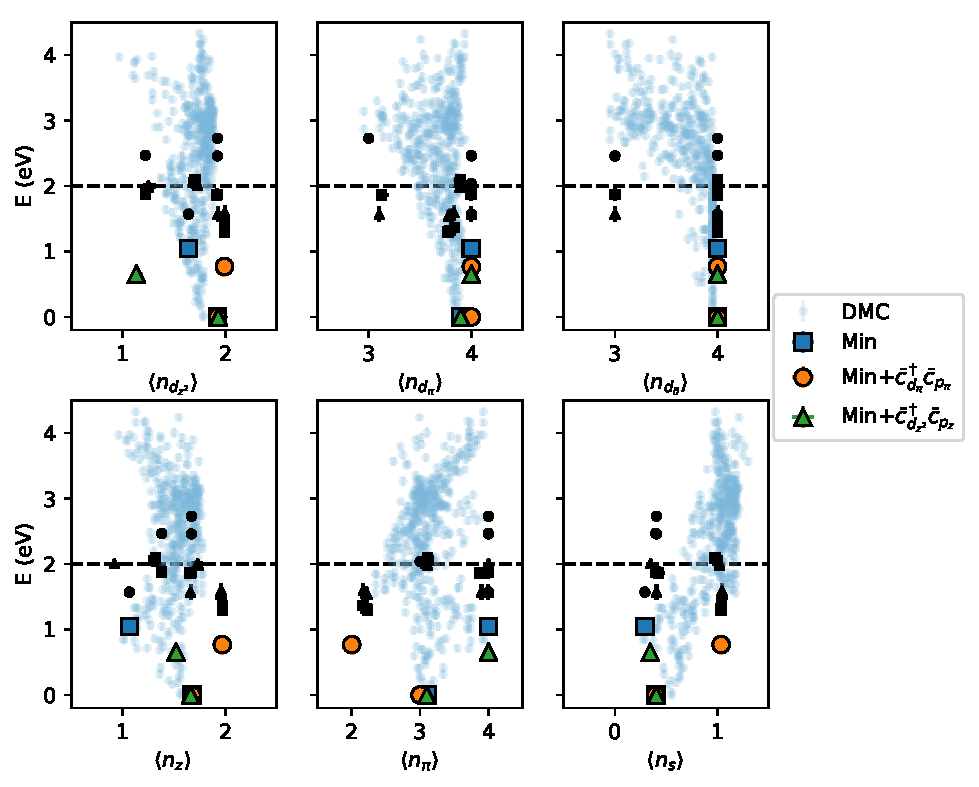
\includegraphics[width=0.45\textwidth]{figs/init_ed.pdf}
	}
	\qquad
	\subfigure[Collection of unique intruder states from our three potential models selected using a k-nearest neighbor approach with k = 5.]{	
		\label{fig:Intruder}
		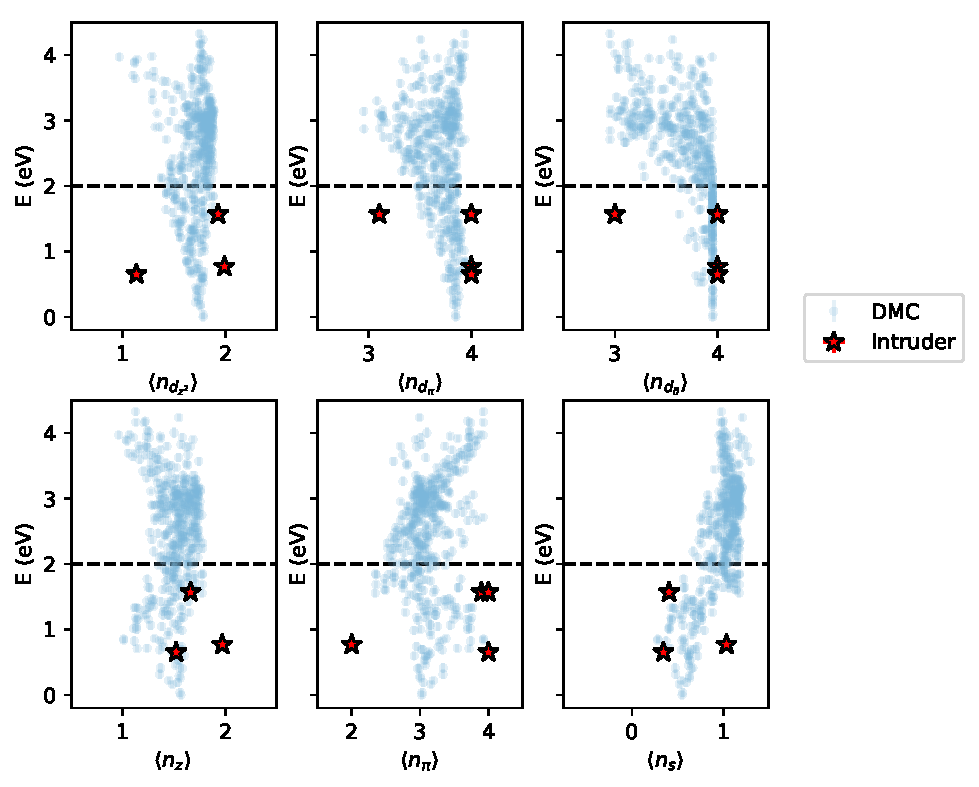
\includegraphics[width=0.45\textwidth]{figs/intruder.pdf}
	}
	\caption{Results of OLS fitting on sampled data and selected intruder states.}
\end{figure}

Given that our intruder states correspond to states within $\mathcal{LE}$ but outside our sample set, they must live within the span of the eigenstates which were excluded in our sampling scheme as described before.
This is evidenced by the fact that two of the intruder states correspond explicitly to excitations we could not access: Cu 3d$_{z^2} \rightarrow $ O 2p$_\pi$ and  Cu 3d$_\pi \rightarrow $ O 2p$_\pi$.
We can approximate these states by single rigid MO excitations above the UKS ground state, which results in states with a FN-DMC energy above 4eV.
Including a generous 2eV reduction in FN-DMC energy due to orbital relaxation, we estimate that these two states should lie at least 2eV in energy. 
Since all the other inaccessible eigenstates are double or higher order excitations, we assert a prior: intruder states should lie above 2eV in energy in our effective theories, enforced via an augmented cost function
\begin{equation}
\text{Cost} = \sum_{i} (E_\text{eff}[\Psi_i] - E_\text{ab}[\Psi_i])^2 + \lambda \sum_{p}\text{QHL}(2 - E_\text{eff}[\Psi_p]),\ \text{QHL}(x) = \Theta(x)x^2
\label{eq:cost}
\end{equation}
where $\lambda>0$ is a parameter which can be varied, QHL is a quadratic hinge loss, $\Theta$ is the Heaviside step function, the index $i$ is over our sampled states and $p$ over the selected intruder states.

\begin{figure}[H]
	\centering
	\subfigure[On the left, scores of the three candidate models at various $\lambda$ when fitting our effective theories using the cost function \eqref{eq:cost}. On the right we show predicted versus calculated energies for our low-energy sampled states for the minimal model fit at $\lambda = 20$.]{
	 	\label{fig:Prior}
		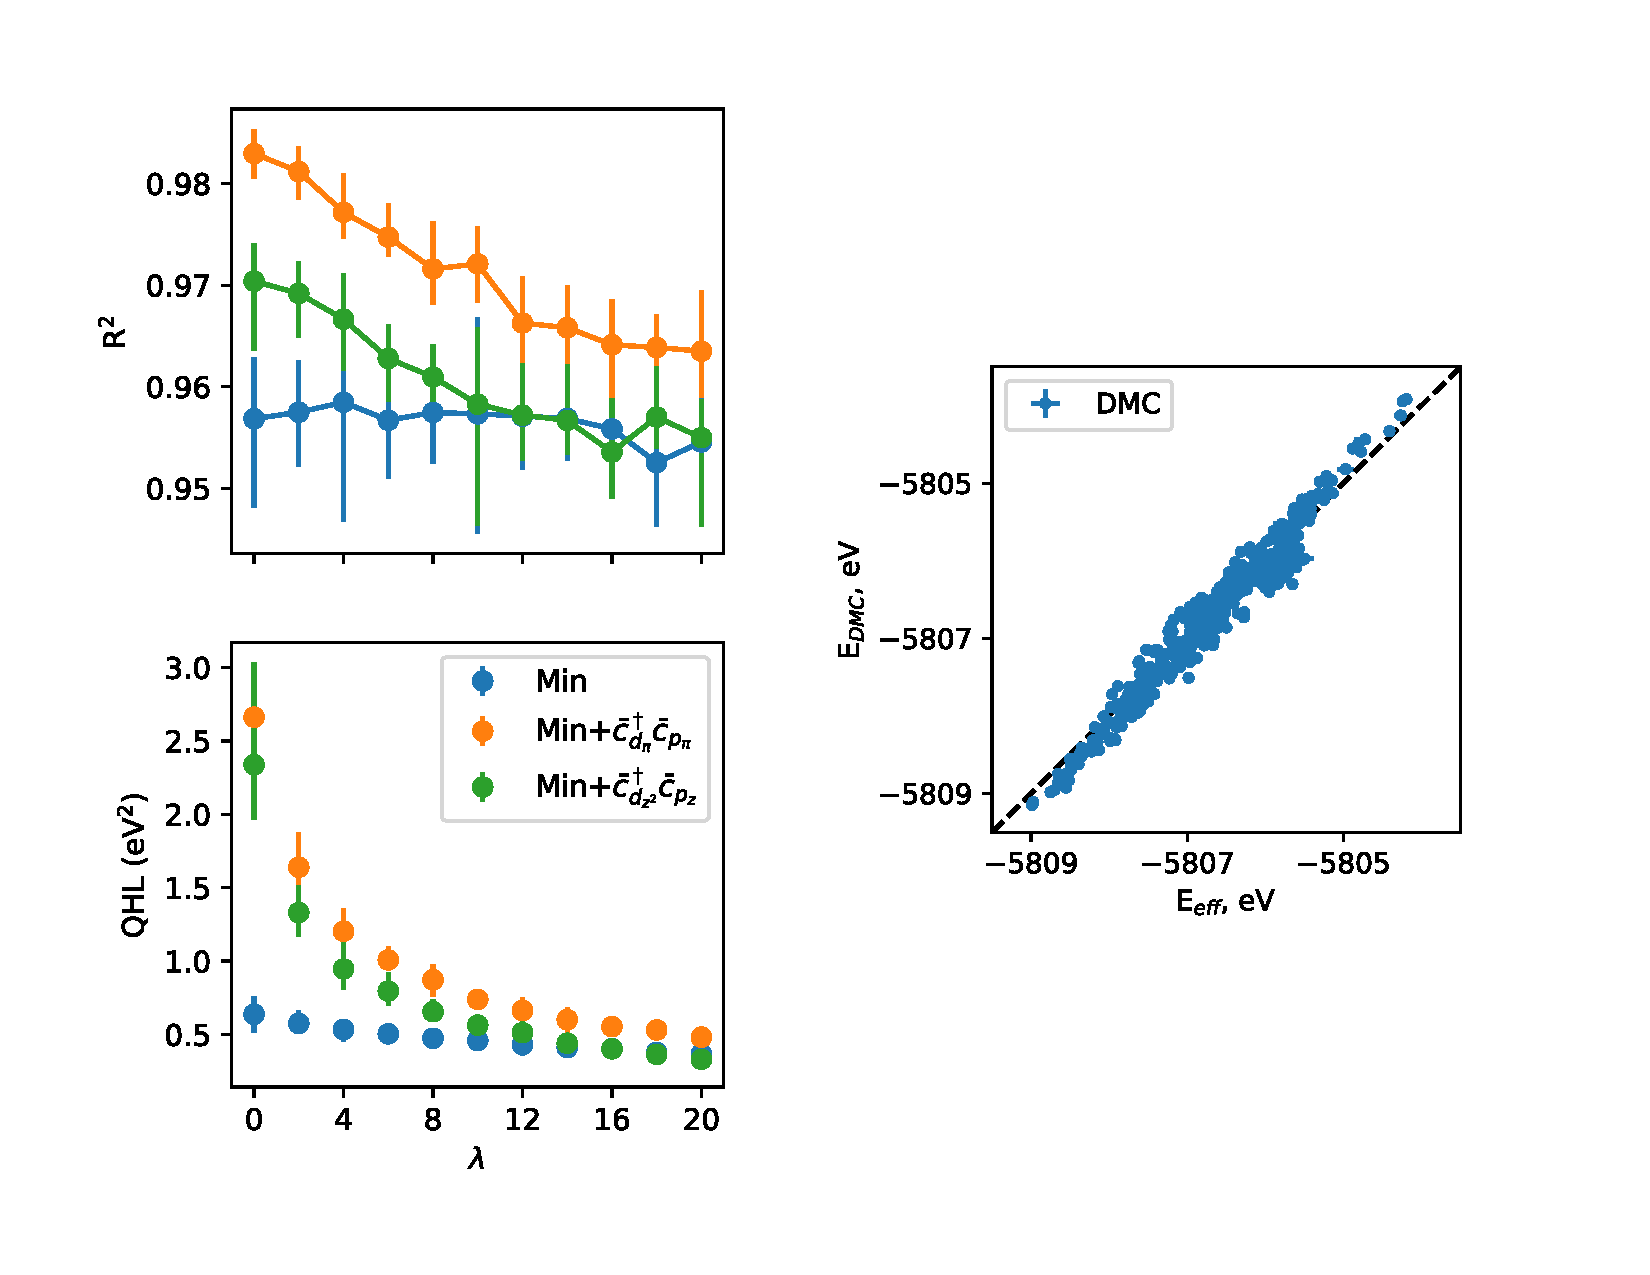
\includegraphics[width=0.45\textwidth]{figs/prior_and_regr.pdf}
	}
	\qquad
	\subfigure[Results of exact diagonalization showing the energies and properties of the first thirty eigenstates for three candidate models using linear regression with cost function \ref{eq:cost} and $\lambda = 20$. The ground state and first excited state are colored and have enlarged markers for clarity. Error bars are 95\% CI calculated by a bootstrap estimate.]{	
		\label{fig:FinalED}
		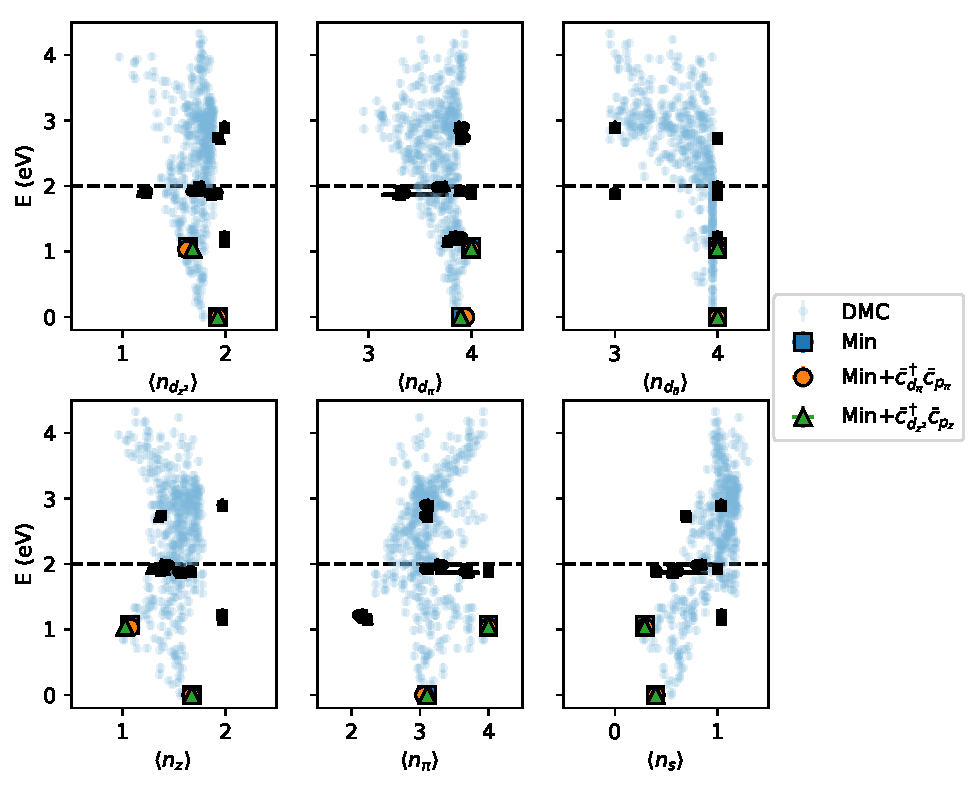
\includegraphics[width=0.45\textwidth]{figs/final_ed.pdf}
	}
	\caption{Results of linear regression using augmented cost function \eqref{eq:cost}.}
\end{figure}

Using our new cost function we find a set of models which accurately describe our sample data, have very similar spectra and eigenvectors to eachother and experiment, and do not contain intruder states below the 2eV prior. 
Shown in Figure \ref{fig:Prior} are the R$^2$ scores and QHL for the three candidate models fit at $\lambda \in [0,20]$. 
We believe that all three models at $\lambda = 20$ should be considered good models as they satisfy our prior and also explain our sample set accurately. 
Also shown are $E_\text{eff}, E_\text{ab}$ for our samples using the minimal model at $\lambda = 20$ to illustrate the high fit quality even with a large $\lambda$.
Figure \ref{fig:FinalED} presents the properties and eigenvalues of the lowest 30 eigenstates for the three fit models at $\lambda = 20$. 
The additional constraint from asserting a prior has seemingly caused a single effective theory to emerge from our set of candidate models.
This conclusion is verified by looking at the values of the fit parameters for our three models, presented in Table 1.
All occupation energies are relative to $\epsilon_{d_\delta}$.
In the doublet sector the ground and first excited state of any of the three models match experiment, as well as the block of states at 2eV corresponding to excitations out of the Cu 3d shell.
The lowest energy quartet states are at 1, 2eV respectively and are in line with the observation of a quartet state at 2eV in APES measurements.

\begin{table}[H]
\begin{center}
\begin{tabular}{l|lllll}
Model &$\epsilon_{d_{z^2}}$ & $\epsilon_{d_\pi}$ & $\epsilon_{4s}$ & $\epsilon_{p_\pi}$ & $\epsilon_{p_z}$ \\ \hline 
Min & 0.32(2)& 0.19(1)& 2.2(4)& 1.7(3)& 0.96(4)\\
Min $ +\ \bar{c}_{d_\pi}^\dagger \bar{c}_{p_\pi}$& 0.32(1)& 0.10(2)& 2.23(3)& 1.8(2)& 0.97(3)\\
Min $ +\ \bar{c}_{d_{z^2}}^\dagger \bar{c}_{p_z}$& 0.29(2)& 0.19(1)& 2.19(5)& 1.7(3)& 0.99(5)\\
\end{tabular} \\

\begin{tabular}{l|llllll}
Model &$t_\pi$ & $t_{dz}$ & $t_{sz}$ & $t_{ds}$ & $J_{sd}$ & $U_s$ \\ \hline 
Min &  -0.57(1)& 0.55(3)& 0.87(2)& 0.44(1)& -0.63(9)& 3.8(2)\\
Min $ +\ \bar{c}_{d_\pi}^\dagger \bar{c}_{p_\pi}$& -0.45(2)& 0.56(2)& 0.89(2)& 0.45(1)& -0.78(7)& 3.7(2)\\
Min $ +\ \bar{c}_{d_{z^2}}^\dagger \bar{c}_{p_z}$& -0.57(1)& 0.54(2)& 0.85(2)& 0.45(2)& -0.58(3)& 3.9(2)\\
\end{tabular} \\

\end{center}
Table 1: Parameters in eV for our three potential models when fit using \eqref{eq:cost} at $\lambda = 20$, energies relative to $\epsilon_{d_\delta} = 0$. Error bars are 95\% CI calculated using a bootstrap estimate.
\end{table}

\section{Proposed work}
My proposed plan involves building a sequence of model Hamiltonians for increasing complicated systems using QMC DMD, working towards an accurate many-body model for TBLG.
The systems I will be interested in are the benzene molecule, single layer graphene, AA stacked bilayer graphene and AB stacked bilayer graphene.
Conceptually, the benzene molecule is a kind of building block for SLG, SLG is a building block for BLG, and BLG for TBLG, creating a sequence of systems from least to most complex.
I do not believe I will be able to build a general model for TBLG in the time span of my thesis, but my work should lay the foundation for further studies using QMC DMD focused on bilayer models with twists.

The first system I will develop a model for is the benzene molecule.
The benzene molecule has chemical formula $C_6 H_6$ and contains a hexagonal ring of carbon atoms with hydrogen atoms sticking out from each carbon.
These carbon atoms are linked by sp$^2$ hybridized $\sigma$ bonds and an alternating sequence of $\pi$ bonds from the C 2p$_z$ orbitals.
Intuitively, the ground state of the system can be seen as a superposition of two configurations of alternating $\pi$ bonds as seen in Figure \textbf{ref} rotated 30$^o$ relative to each other.

While relatively simple, this molecule shares many similarities with and forms the basic unit of SLG.
SLG can be viewed as a tiling of benzene molecules where the external hydrogen legs are replaced by carbon atoms.
The delocalized $\pi$ orbitals in benzene carry over directly into SLG where they are the primary contributors to the well known Dirac bands.
Interaction effects seen in the benzene molecule are also reflected in SLG, such as on-site double occupation energies for the carbon atoms.
As such, developing a model for benzene will help me become familiar with model fitting for 2-D carbon based systems.

The candidate descriptors I will use for DMD are motivated by a previous calculation on the benzene molecule.
In that study, an extended Hubbard model built on the six $\pi$ orbitals was found to perform well in describing the low-lying excitations of the material.
The final model took the form 
\begin{equation}
H_\text{benz} = -\sum_{\langle i,j \rangle} t_{ij}c_i^\dagger c_j + U \sum_i n_{i\uparrow}n_{i\downarrow}  + \sum_{\langle i,j \rangle}V_{ij} n_i n_j + \sum_{\langle \langle i,j \rangle\rangle}V_{ij} n_i n_j
\label{Hbenz}
\end{equation}
where the brackets denote nearest neighbor and next-nearest neighbor summations.
I will consider at least all the descriptors above and also longer range hopping terms.
The single particle orbitals used to express these descriptors will be IAOs.

A new constrained variational Monte Carlo (CVMC) method will be used to sample the low-energy wave functions necessary for DMD.
The CVMC method works by minimizing the following cost function for a parameterized wave function $|\Psi(\vec{p})\rangle$:
\begin{equation}
\vec{p}^* = \text{argmin} \ \langle \Psi(\vec{p}) | \hat{H}_\text{ab} | \Psi(\vec{p}) \rangle - \vec{\lambda} \cdot \langle \Psi(\vec{p}) | (\vec{d} - \vec{d}_0)^2 | \Psi(\vec{p}) \rangle 
\end{equation}
with respect to the parameters $\vec{p}$.
The quantity $\vec{d}$ is short hand for a list of candidate descriptors to sample variations in, $\vec{d}_0$ is the target values of those candidate descriptors, and $\vec{\lambda}$ controls the importance of finding a state with low-energy versus one with descriptor values near $\vec{d}_0$.
Essentially this method allows us, for a given parameterization of $|\Psi(\vec{p})\rangle$, to generate low-energy wave functions which sit near a target point $\vec{d}_0$ in candidate descriptor space.

I will use a multi-Slater-Jastrow (MSJ) parameterization in the CVMC sampling for the benzene molecule.
The multi-Slater expansion will consist of determinants of single particle orbitals calculated using a self consistent field calculation like DFT.
The determinants will include the DFT ground state as well as molecular orbital excitations among the $\pi$ and $\pi^*$ orbitals which form our active space, allowing us to probe variation in all the descriptors above.
A three body Jastrow factor will be applied to ensure that we include correlations in our wave function and that our wave function is low in energy.
The total set of parameters $\vec{p}$ will include both Jastrow and determinental coefficients.

Since a model for benzene has already been developed using DMD, my calculation will also serve as a benchmark for new methods like CVMC sampling.
The CVMC method is relatively new and has not been tested extensively on realistic systems.
The final model that I will produce should be exactly comparable to previous calculations, and as such can give insight into the workings of the CVMC method.
A few questions of interest include whether the CVMC is more statistically efficient in terms of regression, how to select values like $\vec{\lambda}$ and $\vec{d}_0$, and whether the final model fit with CVMC is similar to the one fit previously using a different sampling technique.

The second system I will be interested in working on is SLG.
Single layer graphene is composed of a triangular Bravais lattice with two carbon atoms per unit cell.
In terms of a non-interacting picture, the $\sigma$ orbitals composed of C $2s, 2p_x,$ and $2p_y$ lie below the Fermi level.
The bands which cross the Fermi level, and compose the distinct Dirac cones seen in SLG, are primary $\pi$ bonded molecular orbitals composed of C $2p_z$ orbitals.
The lack of significant screening in SLG leads to long range Coulomb interactions in the system.

The model I am interested in working on will be an extension of a previous model developed for SLG using DMD.
The fit model was a single band, on-site Hubbard model which contained only the $\pi$ orbital degrees of freedom in the system.
The fit model parameters were $U/t \sim$ 2.00, which is smaller than the critical value of $(U/t)_c \sim$ 3.8 for the semimetal-insulator transition in the honeycomb lattice, as expected.
It is interesting to note that if the $\sigma$ orbitals in graphene are treated as a constant negative charge background, then the effective $U$ on site nearly doubles, indicating the importance of including these degrees of freedom in the low-energy sampling.

I will extend the previous model by introducing long range density-density interactions into the effective theory.
As mentioned previously, one expects to see long range Coulomb interactions in graphene due to the vanishing density of states near the Fermi level, in contrast to other metals where electron-hole pairs screen the long range interaction.
I will work on developing a model for SLG of the following form:
\begin{equation}
H_\text{SLG} = -\sum_{i,j} t_{ij}c_i^\dagger c_j + U \sum_i n_{i\uparrow}n_{i\downarrow}  + \sum_{i,j} V_{ij} n_i n_j
\label{Hslg}
\end{equation}
where the indices correspond to the $\pi$ orbitals on the copper atoms, represented by IAO basis elements.
I will consider arbitrarily long range hopping and density-density interaction terms in my model, in contrast to the benzene calculation where the finite size of the system imposes a cutoff in the possible range of interaction.

CVMC will be used to sample the low-energy wave functions necessary to fit the model.
The trial wave function will also be of MSJ type as explained for the benzene molecule, with the determinants built from the single particle orbitals of DFT calculations.
I will consider the DFT ground state determinant and all excitations built on in restricted to the $\pi, \pi^*$ molecular orbitals.
A three-body Jastrow will be used to introduce correlations into the wave function and ensure our sampled states are low in energy.

The last systems I will develop models for are AA and AB stacked BLG.
AA stacked BLG is simply two sheets of graphene placed on top of one another where each atom is aligned with the atom beneath it.
In AB stacked BLG, a carbon atom from the lower layer is present in the center of each carbon hexagon of the upper layer, and vice versa.
As such, one can think of AB BLG as a shifted version of AA BLG, where the shift is half the size of a single carbonic hexagon.

Being the simplest BLG configuration, these models will form a starting point for a more thorough development of models for TBLG.
The ultimate goal of developing a model for TBLG would be a model which has the parameters as a function of the twist angle.
The twist angle changes the local chemistry of a particular atom in a single layer of graphene by introducing neighbors on the other layer at various non-commensurate distances.
As such, the first avenue of investigation would be to see how the model parameters change as one shifts the position of interlayer neighbor carbon atoms. 
The AA and AB BLG configurations provide the simplest systems where this position dependence on model parameters can be probed.

I anticipate that the candidate descriptors should include interlayer couplings as well as the terms seen in SLG.
As such, a candidate model that we may consider initially for BLG would be
\begin{equation}
H_\text{BLG} = H_\text{SLG}^{(1)} + H_\text{SLG}^{(2)} - \sum_{i_1, i_2} t_{i_1, i_2}^\prime c_{i_1}^\dagger c_{i_2} + h.c.
\label{Hblg}
\end{equation}
Here we have two models for the single layers from \eqref{Hslg} plus an interlayer hopping given by the term $t_{i_1, i_2}^\prime.$
I suspect that the hopping values will be very different between the AA and AB models as the distance between interlayer neighbors differs greatly between the two stackings.

I will again use CVMC to generate the low-energy wave functions for the model regression.
As before, I think that an MSJ parameterization will serve the purpose well.
Similarly, the determinants used will include a DFT ground state alongside all excitations within the $\pi, \pi^*$ orbitals of the system.
Note that excitations between the $\pi, \pi^*$ orbitals from both sheets should be included in the multi-Slater expansion.
A three-body Jastrow factor will be used for the reasons listed before.

The final product of my thesis would be four models for these increasingly complex systems.
The model for benzene should reproduce previous results and provide an intro calculation for me, as well as a benchmark test for the CVMC sampling method.
The model for SLG will extend on previous studies, incorporating long range Coulomb interactions.
The models for BLG will be a first step in understanding how interlaying coupling depends on interlayer neighbor distances in the bilayer systems, an important stepping stone towards a general model for TBLG.

Apart from their individual value, the four models can be used to investigate the transferrability of model parameters between these different carbon-based systems.
The first question would be whether the parameter values between a finite size system, like benzene, match those seen in the bulk SLG system.
The second would be whether the intralayer parameter values change in each sheet of SLG when they are brought together in the AA and AB configuration.
The latter question hints at a broader question, whether the SLG intralayer parameters are transferrable to TBLG, especially near the magic twist angles whre interlayer coupling becomes very large.

I conclude by briefly discussing potential avenues of further study in using DMD to develop model Hamiltonians for TBLG. 
One would have to begin by building atomic length scale lattice models for TBLG using DMD, which itself is a monumental task.
When dealing with small commensurate twists, the size of the Moire supercell is enormous and prohibitive to QMC calculations.
As such, a computationally feasible method for probing small shifts, either by translation or angle, between the graphene sheets must be constructed.
This short length scale Hamiltonian can then be downfolded again, using DMD, to a continuum Hamiltonian on the length scale of the Moire superlattice.
This kind of downfolding will require using large-scale tight binding codes like \textbf{ref}.
Iterating over various twist angles can then give insight into the behavior of the long-range effective theory of TBLG as a function of the twist angle.

\subsection{Proposed timeline}
I believe that developing effective theories for the benzene molecule, SLG, AA and AB stacked BLG should take 2 years. 
The model fitting for benzene should take no more than four months.
The goal is to reproduce prior DMD calculations for the same material while benchmarking and familiarizing myself with the new CVMC sampling technique that I will use extensively in my project.
The SLG model fitting should take another eight months.
This is an extension of a previous work, and the first three months will be dedicate to reproducing the results from that work, namely a single band on-site Hubbard model.
Inclusion of long range Coulomb interactions into the effective theory should take another three months.
The last two months will be geared towards finite size extrapolation in order to ensure our final model is applicable to bulk systems.
The last year of the project will be geared towards the AA and AB stacked BLG, with each project taking about six months to complete.
For each stacking, I expect four months will be necessary to build an effective theory, and the final two months will be dedicated to finite size extrapolation.
\end{document}